%!TEX root = ClementiCooperBarba2018.tex

We present results for two kinds of problems. 
The first is a model problem for which an analytical solution is available, 
allowing for a grid-refinement study and code verification using that solution.
It consists of a spherical nanoparticle in a constant electric field, 
where the extinction cross-section can be derived in closed form.
The second set of results use a model for a biosensor detecting a target molecule, 
via frequency shifts in the plasmon resonance of a metallic nanoparticle. 
In this case, since an analytical solution is not available, we can use Richardson 
extrapolation to estimate the errors in a grid-refinement study.
We also computed the variation of the extinction cross-section with respect to wavelength
for the isolated nanoparticle, and in the presence of bovine serum albumin (BSA) proteins, 
varying the location of the analytes.
The final result is a sensitivity study of the biosensor model, 
looking at how the peak in frequency response varies with distance of the protein 
to the nanoparticle.

All results were obtained on a lab workstation, built from parts.
Hardware specifications are as follows: 
\begin{itemize}
  \item CPU: Intel Core i7-5930K Haswell-E 6-Core 3.5GHz LGA 2011-v3
  \item RAM: G.SKILL Ripjaws 4 series 32GB (4 x 8GB)
  \item GPU: Nvidia Tesla K40c (with 12 GB memory)
\end{itemize}

\subsection{Grid convergence and verification with an isolated silver nanoparticle} \label{sec:verification}

\noindent In the long-wavelength limit, the electrostatic approximation applies and
the electromagnetic scattering of a small spherical particle can be modeled
by a sphere in a constant electric field. 
Figure \ref{fig:np_elec_field} illustrates this scenario.

%
\begin{figure}[h] %  figure placement: here, top, bottom, or page
   \centering
   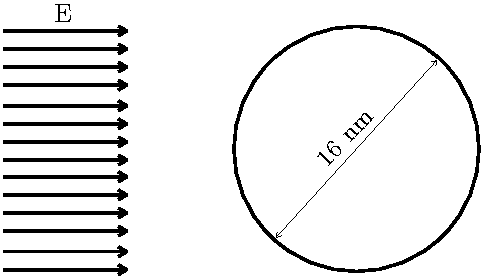
\includegraphics[width=0.3\textwidth]{sphere_field_8nm.pdf} 
   \caption{Spherical nanoparticle in a constant electric field.}
   \label{fig:np_elec_field}
\end{figure}
%

This model problem has an analytical solution, which allows us to compare with
the numerical calculations of the extinction cross-section obtained with \pygbe,
for code verification and grid-convergence analysis.
Mishchenko \cite{Mishchenko2007} derived the following analytical result, 
valid for lossy mediums:
%
\begin{equation} 
    C_\text{ext} = \frac{4\pi a^3}{k^\prime} \operatorname{Im}\left(k^2 
                    \frac{\epsilon_p/\epsilon_m -1}{\epsilon_p/\epsilon_m +2}\right).
    \label{eq:an_sol}
\end{equation}
%
Here, $a$ is the radius of the sphere, $k$ is the complex wave number ($k=k^\prime +i k^{\prime\prime}$), $\epsilon_p$ 
is the dielectric constant of the particle, and $\epsilon_m$ is the dielectric constant
of the host medium. If the medium is not lossy, then $k^{\prime\prime}=0$ and $k=k^\prime$.

We completed a grid-convergence study of \pygbe for the extinction
cross-section of a spherical silver nanoparticle of radius 8 nm immersed in water,
under a $z$-polarized electric field with a wavelength of 380 nm and intensity of 
$-0.0037 e/({\AA}^2 \, \epsilon_0)$. In these conditions, water has a dielectric
constant of $1.7972 \, + \, 8.5048^{-09}i$ \cite{JohnsonChristy1972} and silver of
$-3.3877 \, + \, 0.1922i$ \cite{HaleQuerry1972}. 
Table \ref{table:quadparams1} lists the Gauss quadrature points used for each type of boundary element. 
The threshold parameter defining the near-singular region was 0.5 
(refer to the \pygbe documentation, under ``Parameter file format'').
Table \ref{table:treeparams1} shows the treecode and solver parameters for this grid-convergence study.

\begin{table}[h]
    \centering
    \caption{\label{table:quadparams1} Grid-convergence study: Gauss quadrature points; 
    $K$ and $K_{fine}$ are per element; $N_k $ is per element edge (semi-analytical integration). } 
    \begin{tabular}{l l}
    \hline%\toprule
     distant elements: & $K=4$ \\
     near-singular integrals:   & $ K_{fine}=37$ \\
     singular elements:  & $N_k =9$ \\
    \hline%\bottomrule
    \end{tabular}
\end{table}


\begin{table}[h]
    \centering
    \caption{\label{table:treeparams1} Grid-convergence study: treecode and solver parameters.} 
    \begin{tabular}{l l}
    \hline%\toprule
    treecode order of expansion: & $P=15$\\
    MAC                                         & $\theta=0.5$\\
    GMRES tolerance                    & $10^{-5}$\\
    \hline%\bottomrule
    \end{tabular}
\end{table}

The results are shown in Figure \ref{fig:error_sphere_Ag}, where the mesh sizes are
512, 2048, 8192, and 32768 elements. 
The analytical solution with equation \eqref{eq:an_sol} is $C_{ext} = 1854.48$ nm$^2$, 
and the computed errors are as shown in Table \ref{table:err_iso_sphere}.
The dashed line in Figure \ref{fig:error_sphere_Ag} shows a $1/N$ slope, 
and the observed order of convergence is $0.98$,  
evidence that the meshes are correctly resolving the numerical solutions with \pygbe. 


\begin{figure}[h] %  figure placement: here, top, bottom, or page
   \centering
   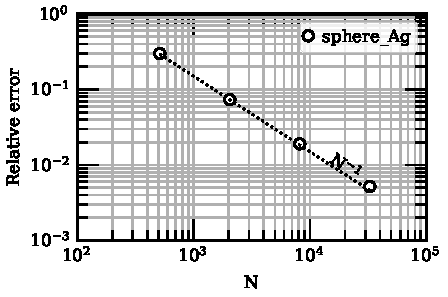
\includegraphics[width=0.45\textwidth]{convergence_sph_Ag_R8_w=380.pdf} 
   \caption{Grid-convergence study for the extinction cross-section of a spherical silver
            nanoparticle, computed with \pygbe. Figure, plotting script and auxiliary files available under \textsc{cc-by} \cite{ClementiETal2018c}.}
   \label{fig:error_sphere_Ag}
\end{figure}



\begin{table}[h]
    \centering
    \caption{\label{table:err_iso_sphere} Percentage error in the grid-convergence cases with an isolated silver nanosphere.} 
    \begin{tabular}{c c}
    \hline%\toprule
    N & \% error \\
    \hline%\midrule
     $512$ & $29.86$ \\
     $2048$ & $7.33$ \\
     $8192$ & $1.9$ \\
     $32768$ & $0.52$ \\
    \hline%\bottomrule
    \end{tabular}
\end{table}

As another verification test of \pygbe in the LSPR setting, we computed the extinction cross-section of an 
isolated sphere for a range of wavelengths. 
The results are shown in Figure \ref{fig:verif_sphere}, comparing with the analytical solution. 
The values of the dielectric constant for each wavelength were obtained by interpolation of 
experimental data \cite{JohnsonChristy1972, HaleQuerry1972}.
For reproducibility of these results, we provide a Jupyter notebook with the code used for this interpolation step.
See section \ref{sec:repro} for details.
We used a mesh with $N=32768$, and relaxed some parameters compared with the grid convergence results shown previously, still yielding errors below $1\%$ at all frequencies.
The parameters used are shown in Tables \ref{table:quadparams2} and \ref{table:treeparams2}.
Figure \ref{fig:verif_sphere} shows good agreement between the computed and analytical results, 
evidence that \pygbe can accurately represent the mathematical model. 


\begin{table}[h]
    \centering
    \caption{\label{table:quadparams2} Verification: Gauss quadrature points; 
    $K$ and $K_{fine}$ are per element; $N_k $ is per element edge (semi-analytical integration). } 
    \begin{tabular}{l l}
    \hline%\toprule
     distant elements: & $K=4$ \\
     near-singular integrals:   & $ K_{fine}=19$ \\
     singular elements:  & $N_k =9$ \\
    \hline%\bottomrule
    \end{tabular}
\end{table}


\begin{table}[h]
    \centering
    \caption{\label{table:treeparams2} Verification: treecode and solver parameters.} 
    \begin{tabular}{l l}
    \hline%\toprule
    treecode order of expansion: & $P=6$\\
    MAC                                         & $\theta=0.5$\\
    GMRES tolerance                    & $10^{-3}$\\
    \hline%\bottomrule
    \end{tabular}
\end{table}


\begin{figure}[h] %  figure placement: here, top, bottom, or page
   \centering
   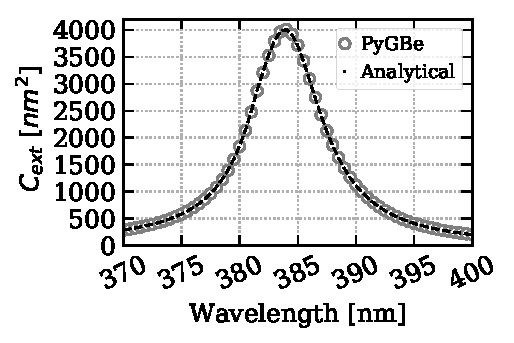
\includegraphics[width=0.45\textwidth]{silver_NP_verification.pdf} 
   \caption{Extinction cross-section as a function of wavelength for an $8$-nm
            silver sphere immersed in water. The peak in the values of extinction cross-section corresponds to the plasmon resonance of the metallic nanoparticle under the incoming electric field. Figure, plotting script and auxiliary files available under \textsc{cc-by} \cite{ClementiETal2018d}.}
   \label{fig:verif_sphere}
\end{figure}




\subsection{LSPR response to bovine serum albumin (BSA)} \label{sec:lspr_response}

Localized Surface Plasmon Resonance (LSPR) biosensors detect a target molecule by monitoring
frequency shifts in the plasmon resonance of metallic nanoparticles, in presence of an analyte \cite{WilletsVandyune2007}.
In this section, we model the response of LSPR biosensors using the expanded capacity of \pygbe.
We consider a spherical silver nanoparticle, and compute the extinction cross-section placing 
bovine serum albumin (BSA) proteins (PDB code: 4FS5) in different locations.
The BSA surface mesh was generated using the open-source software Nanoshaper \cite{Nanoshaper}. 
Nanoshaper takes as inputs the atomic coordinates and radii, which were 
extracted from a \texttt{pqr} file generated with \texttt{pdb2pqr} \cite{Dolinsky04},
 using the built-in \texttt{amber} force field.
 In support of the reproducibility of our results, we deposited the final meshes in the Zenodo data repository.
See section \ref{sec:repro} for details.

\subsubsection{Grid-convergence study} \label{sec:bsa_convergence}
We performed a grid-convergence 
analysis of the system sketched in Figure \ref{fig:setup_conv}. 
Since we compute the extinction cross-section of the spherical nanoparticle only, we 
set a fixed mesh density for the protein and refined the mesh of the
sphere (meshes of 512, 2048, 8192 and 32768 elements). We found that the protein meshed with two
triangles per ${\AA}^2$ was fine enough for the convergence analysis, resulting in $N_{prot} = 98116$ elements. 


\begin{figure}[h] %  figure placement: here, top, bottom, or page
   \centering
   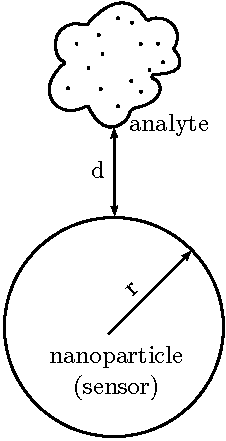
\includegraphics[width=0.15\textwidth]{protein_sphere_sketch.pdf} 
   \caption{Setup for convergence analysis of the LSPR response calculations.}
   \label{fig:setup_conv}
\end{figure}

We used the same physical conditions as in the grid convergence with an isolated silver nanoparticle, and the same numerical parameters, presented in Tables \ref{table:quadparams1} and \ref{table:treeparams1}.
For the protein dielectric constant, we used $2.7514 + 0.2860i$, obtained from the 
functional relationship provided by Phan, et al.~\cite{PhanETal2013}.
The distance between the sensor and the analyte was $d=1$ nm, 
and the BSA protein was oriented such that its dipole moment was aligned with the $y$-axis. 
To obtain the error estimates shown in Figure \ref{fig:error_sphere-bsa} and Table \ref{table:err_bsa_sensor},
we used the Richardson extrapolated value of extinction cross-section as a reference, 
$C_{ext}= 1778.73$ nm$^2$.


\begin{figure}[h] %  figure placement: here, top, bottom, or page
   \centering
   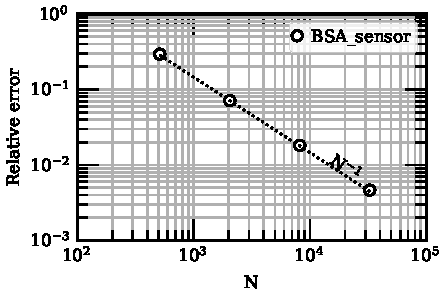
\includegraphics[width=0.45\textwidth]{convergence_bsa_sensor_R8_d=1_w=380.pdf} 
   \caption{Grid-convergence study of extinction cross-section of a spherical silver
            nanoparticle with a BSA protein at $d=1$ nm. Figure, plotting script and auxiliary files available under \textsc{cc-by} \cite{ClementiETal2018c}.}
   \label{fig:error_sphere-bsa}
\end{figure}

The observed order of convergence is $0.99$, and 
Figure \ref{fig:error_sphere-bsa} shows that the error decays with the number
of boundary elements ($1/N$), which is consistent with our verification 
results in Section \ref{sec:verification}. This provides evidence that the
numerical solutions computed with \pygbe are correctly resolved by the meshes.
The percentage errors for the different meshes are presented in Table \ref{table:err_bsa_sensor}.

\begin{table}%[h]
    \centering
    \caption{\label{table:err_bsa_sensor} Estimated percentage error of the BSA-sensor system (Fig.~\ref{fig:setup_conv}), with respect to the extrapolated value (using Richardson extrapolation).} 
    \begin{tabular}{c c}
    \hline%\toprule
    N & \% error \\
    \hline%\midrule
     $512$ & $29.39$ \\
     $2048$ & $7.13$ \\
     $8192$ & $1.82$ \\
     $32768$ & $0.46$ \\
    \hline%\bottomrule
    \end{tabular}
\end{table}

\subsubsection{Resonance frequency shift} \label{sec:bsa_shift}

We computed the LSPR response as a function of the wavelength in the presence 
of the BSA protein. To optimize run-times without compromising accuracy, we used a relaxed
set of parameters, where the protein mesh density was one element per
${\AA}^2$ ($N_{prot}=45140$) and the sphere mesh had $N_{sensor}=32768$ elements. 
These calculations used the same parameters as shown in Tables \ref{table:quadparams2} and \ref{table:treeparams2}.
This parameter choice resulted in a percentage error below 1\%, with respect to the Richardson-extrapolated value.
The run time for each one of these cases was approximately $7.5$ min using one NVIDIA Tesla K40c GPU. 
When two proteins are present, the run time per case is approximately  $15$ min. 

\begin{center}
\begin{figure*}[t] %  figure placement: here, top, bottom, or page
   \centering
   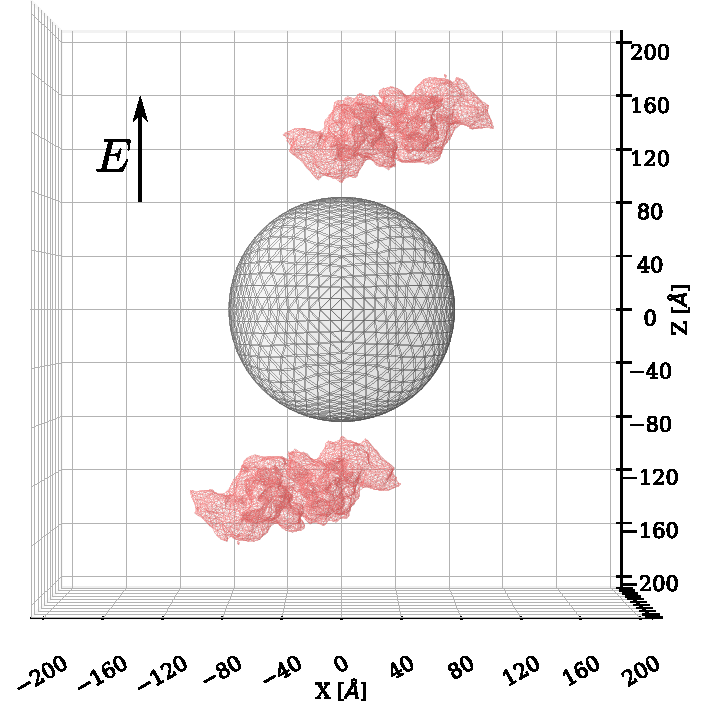
\includegraphics[width=0.65\textwidth]{2prot_1nm_z_R8nm.pdf} 
   \caption{Sensor protein display: BSA located at $\pm 1$ nm of the 
            nanoparticle in the $z$-direction. Figure, plotting script and auxiliary files available under \textsc{cc-by} \cite{ClementiETal2018e}.}
   \label{fig:display_z}
\end{figure*}
\end{center}

Figure \ref{fig:display_z} shows a visualization of the meshes for these calculations, 
with two BSA proteins placed at a distance $d=1$ nm away from a spherical silver nanoparticle, along the $z$-axis.
The surface-mesh data, plotting scripts and figure are available openly on Figshare, 
in support of the paper's reproducibility\cite{ClementiETal2018e}.
The position of the BSA molecule in the $+z$ axis was the same as in the convergence analysis in 
Section \ref{sec:bsa_convergence}, whereas the BSA in the $-z$ position is a 180$^\circ$ 
solid rotation  about the $y$-axis of the BSA in $+z$.
We performed calculations for wavelengths between $382$ nm and $387$ nm, every $0.25$ nm,
which are around the peak seen in Figure \ref{fig:verif_sphere}.

Figure \ref{fig:2pz_response} shows the variation of the extinction cross-section
with respect to wavelength for the isolated nanoparticle ($d=\infty$) and with
BSA proteins placed $d=1$ nm away. 
The result shows a red-shift ($0.5$ nm) in the resonance frequency due to the
presence of the BSA analytes.


\begin{figure}[h] %  figure placement: here, top, bottom, or page
   \centering
    %since we have dots in the names we need to enclose what is before the 
    %extension in { }
   \includegraphics[width=0.45\textwidth]{{2pz_00_ef-0.0037_R8nm}.pdf} 
   \caption{Extinction cross-section as a function of wavelength for a $8$ nm
            silver sphere immersed in water with two BSA proteins placed at
            $\pm 1$ nm away from the surface in the $z$-direction, and at
            infinity (no protein).}
   \label{fig:2pz_response}
\end{figure}

\begin{figure}[t] %  figure placement: here, top, bottom, or page
   \centering
   \subfloat{\includegraphics[width=0.45\textwidth]{{2px_00_ef-0.0037_R8nm}.pdf}}\\
   \subfloat{\includegraphics[width=0.45\textwidth]{{2py_00_ef-0.0037_R8nm}.pdf}} 
   \caption{Extinction cross-section as a function of wavelength for an $8$-nm
            silver sphere immersed in water with two BSA proteins placed at
            $\pm 1 $ nm away from the surface in the $x$-direction (top) and
             $y$-direction (bottom), and at infinity (no protein).}
   \label{fig:2pxy_response}
\end{figure}

To study the effect of location of the analytes, we re-computed the result placing the 
BSA proteins along the $x$- and $y$-axis, at $\pm 1$ nm, as shown in Figure \ref{fig:display_xy}.
These configurations were obtain by performing a solid rotation of the z-configuration (Figure
\ref{fig:display_z}) of 90 degrees along the $x$- and $y$-axis respectively.
Figure \ref{fig:2pxy_response} shows the results, in each case.  


\subsubsection{Sensitivity calculations} \label{sec:bsa_sensitivity}

The sensitivity of an LSPR biosensor corresponds to the relationship between the size 
of the resonance frequency shift and the number of analytes bound to the sensor (through a ligand).
Experiments show that the distance between the nanoparticle and the analyte 
affects the sensitivity of the sensor, to the point that
targets placed $15$ nm away from the surface are very hard to detect \cite{HaesETal2004}.
This is a critical issue, considering that common ligands (for example, antibodies) are
larger than $15$ nm. Figure \ref{fig:dist_response} 
shows how the peak varies with the distance at which the analytes ($+z$ and $-z$) are placed.  
In particular, we see a shift of $0.25$ nm when $d=2$ nm to $0.75$ nm when the 
analytes are placed at $d=0.5$ nm. The parameters used in this case remain 
the same as the ones used in Figures \ref{fig:2pz_response} and \ref{fig:2pxy_response} .


\begin{figure}%[h] %  figure placement: here, top, bottom, or page
   \centering
   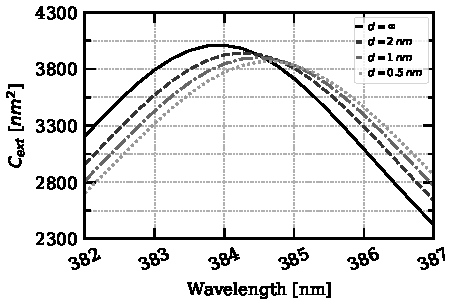
\includegraphics[width=0.45\textwidth]{2pz_lspr_response.pdf} 
   \caption{Extinction cross-section as a function of wavelength for an $8$-nm
            silver sphere immersed in water with two BSA proteins placed at
            $2$, $1$, and $0.5$ nm away from the surface in the 
            $z$-direction, and at infinity (no protein).}
   \label{fig:dist_response}
\end{figure}




\begin{figure*}
   \centering
   \subfloat{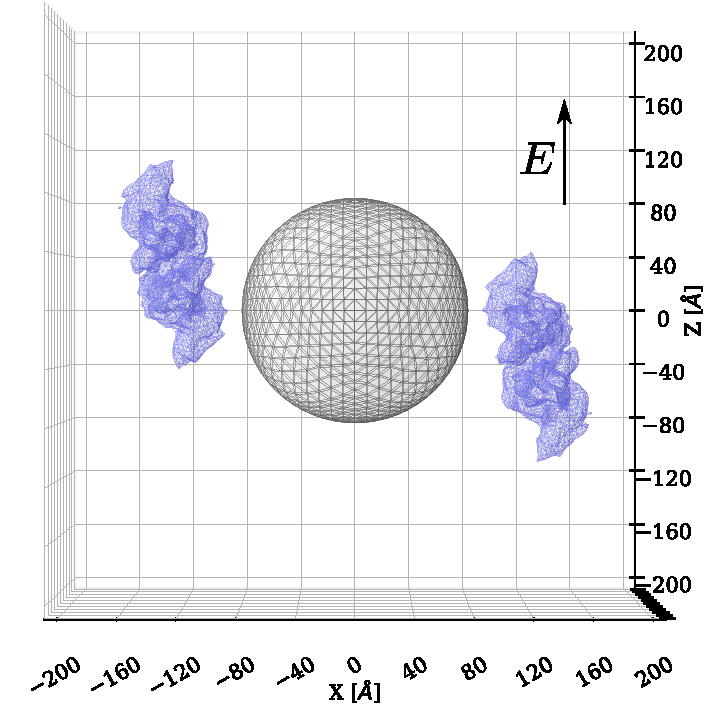
\includegraphics[width=0.65\textwidth]{2prot_1nm_x_R8nm.pdf}} \\
%   \caption{Sensor protein display: BSA located at 1 nm of the nanoparticle in the
%            $x$-direction}
%   \label{fig:display_x}
%\end{figure*}
%
%\begin{figure*}
\vspace{-0.5cm}
   \subfloat{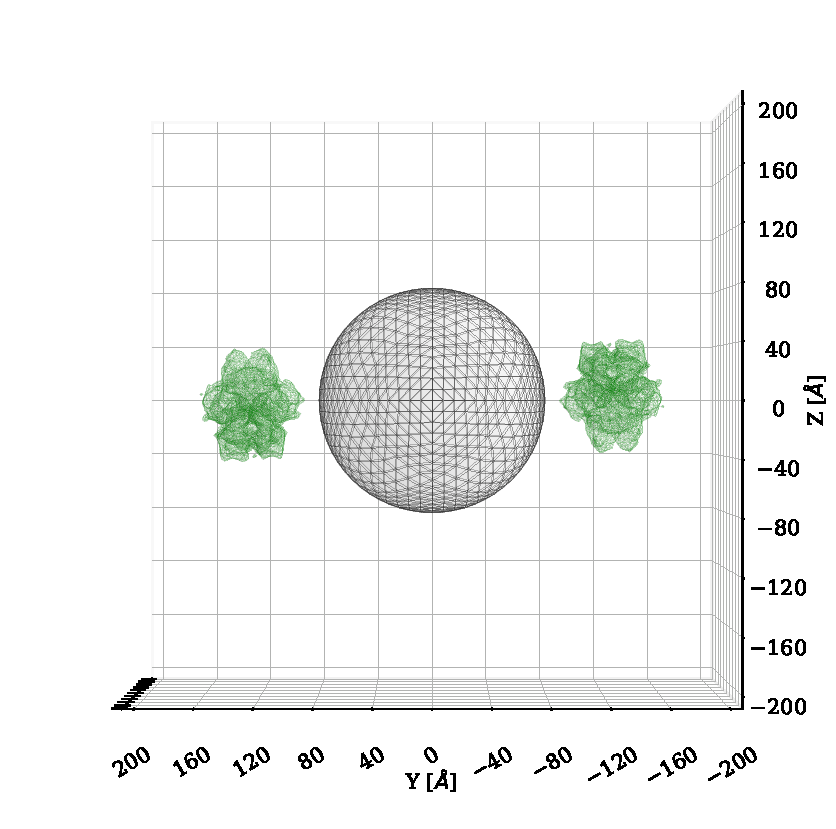
\includegraphics[width=0.65\textwidth]{2prot_1nm_y_R8nm.pdf}} 
%   \caption{Sensor protein display: BSA located at 1 nm of the nanoparticle in the
%            $y$-direction}
    \caption{Sensor protein display: BSA located at $\pm 1$ nm of the nanoparticle in the
           $x$-direction (top) and $y$-direction (bottom). Figure, plotting script and auxiliary files available under \textsc{cc-by} \cite{ClementiETal2018e}.}
    \label{fig:display_xy}
\end{figure*}


\subsection{Reproducibility and data management} \label{sec:repro}

To facilitate the reproducibility and replication of our results, 
we consistently release our research code and data with every publication. \pygbe is openly developed and 
shared under the BSD3-clause license via its repository at \url{https://github.com/barbagroup/pygbe}.

We also release all of the data and scripts needed to run the calculations reported in this work, 
as well as the post-processing scripts to reproduce the figures in this paper. 
All the input files necessary to reproduce the computations are available in one Zenodo data set \cite{ClementiETal2018a}. 
Each problem corresponds to a folder, wherein the user can find geometry files (surface meshes), 
configuration files, parameter files, and when it applies, the protein charges (.pqr).
The scripts and auxiliary files needed to run \pygbe to re-generate every result in the paper are collected in another Zenodo deposit \cite{ClementiETal2018b}.
After execution, the resulting data needed to re-create the figures in the paper will be saved in the running folder and the input files (the first Zenodo set) can at that point be deleted.
(For more details, the reader can consult a README file in the Zenodo archive.)
\emph{Reproducibility packages} to reproduce the figures in the paper are deposited on Figshare, 
including the figures, plotting scripts and a Jupyter notebooks that organize and re-create the results \cite{ClementiETal2018c,ClementiETal2018d,ClementiETal2018e,ClementiETal2018f}.
